% ------------------------------------------------------------------------------
% TYPO3 Version 10.2 - What's New (French Version)
%
% @license	Creative Commons BY-NC-SA 3.0
% @link		http://typo3.org/download/release-notes/whats-new/
% @language	French
% ------------------------------------------------------------------------------

\section{Interface Utilisateur Backend}
\begin{frame}[fragile]
	\frametitle{Interface Utilisateur Backend}

	\begin{center}\huge{Chapitre 1~:}\end{center}
	\begin{center}\huge{\color{typo3darkgrey}\textbf{Interface Utilisateur Backend}}\end{center}

\end{frame}

% ------------------------------------------------------------------------------
% Feature | 89458 | Show link to online docs in extension manager

\begin{frame}[fragile]
	\frametitle{Interface Utilisateur Backend}
	\framesubtitle{Gestionnaire d'extensions}

	Le gestionnaire d'extension affiche les liens vers la document des extensions.

	\begin{figure}
		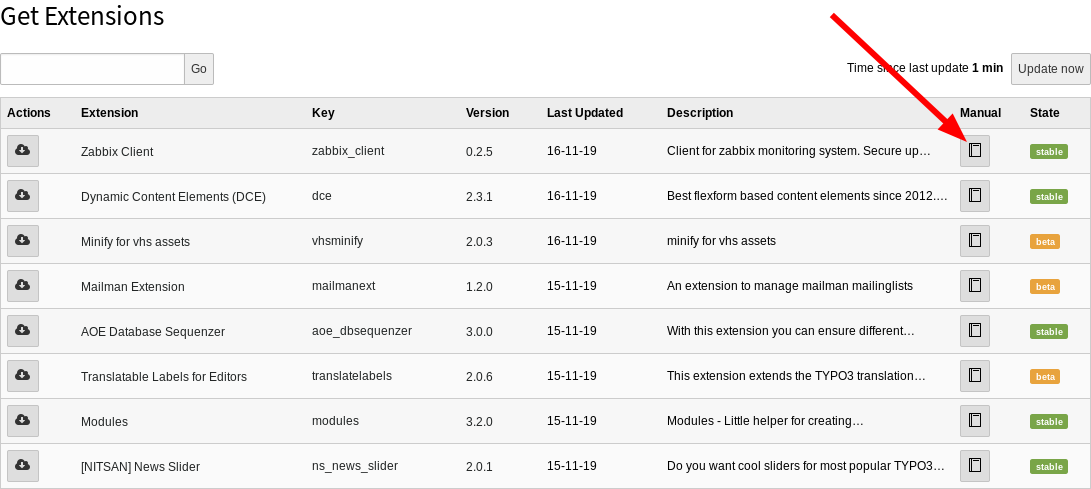
\includegraphics[width=0.90\linewidth]{ChangesForIntegrators/89458-ShowLinkToOnlineDocsInExtensionManager.png}
	\end{figure}

\end{frame}

% ------------------------------------------------------------------------------
% Feature | 86818 | Reintroduce keyboard accessible version of the pagetree

\begin{frame}[fragile]
	\frametitle{Interface Utilisateur Backend}
	\framesubtitle{Accessibilité de l'arborescence des pages}

	Les utilisateurs Backend peuvent naviguer au clavier dans l'arborescence des pages.
	En utilisant les flèches, «~début~», «~fin~», «~entrer~», «~espace~», etc.
	\newline
	Ceci en accord avec les bonnes pratiques décrites dans
	\href{https://www.w3.org/TR/wai-aria-practices-1.1/#keyboard-interaction-22}{WAI-ARIA Authoring Practices 1.1 (en)}
	par le W3C.

	\begin{figure}
		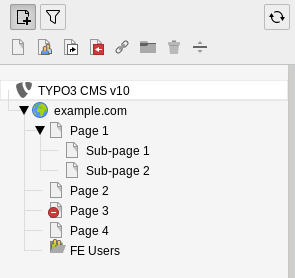
\includegraphics[width=0.30\linewidth]{BackendUserInterface/86818-PagetreeAccessibility.png}
	\end{figure}

\end{frame}

% ------------------------------------------------------------------------------
